\chapter{Optical Properties of Linear Anisotropic Media}
\section{Optical Classification of Anisotropic Media}
On peut trouver les propriétés de propagation de trois façons différentes : la surface normale, 
Fresnel et l'ellipsoid index. On détermine ça via le tenseur dielectrique via les indices principaux 
de réfraction $n_1, n_2$ et $n_3$. On a également vu que pour les axes principaux, il n'y avait pas 
de biréfringence. Une classification logique est de procéder par nombre d'axes optiques : deux 
est le cas le plus général mais il peut y en avoir un ou zéro selon le degré de symétrie, ou encore 
une infinité (tout est axe optique)\footnote{Voir pages 73-74}. 

\subsubsection{Cristaux bi-axiaux}
Le cas le plus général, avec le moins de symétries : deux axes optiques. Par convention on utilise le
système de coordonnées tel que $n_1 < n_2 < n_3$. Avec cette convention, les deux axes optiques sont
situés dans le plan $xz$.

\subsubsection{Cristaux uniaxial}
Lorsque deux indices principaux sont égaux, il n'y a que un axe optique. Les deux indices égaux sont
nommé \textit{indice ordinaire} et l'autre \textit{extra-ordinaire}
\begin{equation}
n_1=n_2=n_0\qquad\qquad;\qquad\qquad n_3=n_e
\end{equation}
On peut alors factoriser la surface normale telle que
\begin{equation}
\left(\dfrac{k_x^2+k_y^2}{n_e^2}+\dfrac{k_z^2}{n_o^2}-\dfrac{\omega^2}{c^2}\right)\left(\dfrac{k^2}{n_o^2}
-\dfrac{\omega^2}{c^2}\right)=0
\end{equation}
La surface normale est donc une sphère et une ellipsoïde de révolution, il n'y a bien qu'un axe optique.
\begin{center}
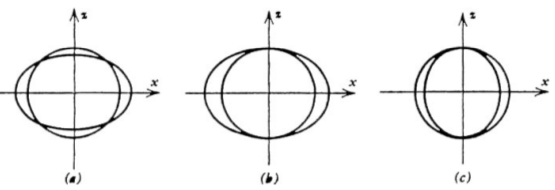
\includegraphics[scale=0.75]{ch5/image1}
\captionof{figure}{Surface normale pour (a) biaxial, (b) uniaxial positif et (c) uniaxial négatif}
\end{center}

\subsubsection{Cristal isotropique}
Tous les indices sont égaux, la surface normale se dégénère en une sphère.

\section{Light Propagation in Uniaxial Crystals}
Un tel cristal est vraiment cher, il n 'y a en effet pas besoin de "chercher" l'axe optique ce qui n'est
pas le cas pour les cristaux biaxiaux. 

\subsection{Theory of Light Propagation in Uniaxial Crystals}
Par convention, on défini l'axe $z$ comme axe de symétrie de sorte à ce que l'index ellipsoid s'écrive
\begin{equation}
\dfrac{X^2+Y^2}{n_o^2}+\dfrac{Z^2}{n_e^2}=1
\end{equation}
Par invariance de rotation autour de $z$, on peut choisir le système de coordonnées tel que la direction
de propagation soit dans le plan $yz$. On définira $\theta$ comme l'angle entre la direction de propagation
et l'axe $z$.

\subsubsection{La surface normale}
En substituant
\begin{equation}
k_z = \dfrac{\omega}{c}n\cos\theta,\qquad\qquad k_x=0,\qquad\qquad k_y=\dfrac{\omega}{c}n\sin\theta
\end{equation}
L'équation \eqref{eq:4.19} devient
\begin{equation}
\left(\begin{array}{ccc}
n_o-n^2 & 0 & 0\\
0 & n_o^2-n^2\cos^2\theta & n^2\sin\theta\cos\theta\\
0&n^2\sin\theta\cos\theta & n_e^2-n^2\sin^2\theta
\end{array}\right)\left(\begin{array}{c}
E_x\\
E_y\\
E_z
\end{array}\right)=0
\end{equation}
Cette expression est identique à la précédente, mais écrit avec des fonctions trigonométriques dans le
cas d'un cristal uniaxial. Il est évident que pour chaque direction de propagation, il y a un mode 
propre d'indice de réfraction $n_o$ polarisé selon l'axe $x$. On trouve le second indice de réfraction
(du second mode propre) en résolvant
\begin{equation}
\left|\begin{array}{cc}
n_o^2-n^2\cos^2\theta & n^2\sin\theta\cos\theta\\
n^2\sin\theta\cos\theta & n_e^2-n^2\sin^2\theta
\end{array}\right| = 0
\end{equation}
On peut résoudre cette équation pour l'indice de réfraction
\begin{equation}
n^{(2)} = \left(\dfrac{\cos^2\theta}{n_o^2}+\dfrac{\sin^2\theta}{n_e^3}\right)^{-\frac{1}{2}}
\end{equation}
qui donne l'indice de réfraction du second mode propre comme une fonction de $\theta$. Il s'agit de la même
équation que précédemment, juste notée en $f(\sin,\cos)$. Quelques cas particuliers
\begin{description}
\item[$\theta=0$] $n^{(2)}=n_e$, polarisé linéairement en $y$
\item[$\theta=\pi/2$] $n^{(2)}=n_e$, polarisé linéairement en $z$
\item[$\theta$] $n^{(2)}\in [n_e,n_o]$ ou $n^{(2)}\in [n_e,n_o]$ 
\end{description}
Le champ électrique est donné par
\begin{equation}
E^{(2)} = E_0\left(\dfrac{\sin^2\theta}{n^{(2)2}-n_o^2}+\dfrac{\cos^2\theta}{n^{(2)2}-n_e^2}\right)
\end{equation}
Ce qui n'est pas perpendiculaire à la direction de propagation, sauf pour $\theta = 0, \pi/2$. Par
contre, les deux modes propres sont \textbf{orthogonaux}\footnote{Perpendiculaires l'un à l'autre} mais
\textbf{pas transverse}\footnote{Perpendiculaire à la direction de propagation}
\begin{equation}
\cos(s,E^{(2)}) \neq 0
\end{equation}


\subsubsection{The index ellipsoid}
On peut en tirer les mêmes conclusions avec l'approche de l'index ellipsoid quia pour équation
\begin{equation}
\dfrac{X^2+y^2}{n_o^2}+\dfrac{Z^2}{n_e^2}=1
\end{equation}
Le principe reste mathématique (voir page 79) et permet de trouver
\begin{equation}
\dfrac{1}{n^{(2)2}} = \dfrac{\cos^2\theta}{n_o^2}+\dfrac{\sin^2\theta}{n_e^2}
\end{equation}








\section{Refraction at a boundary}
\subsection{Double Refraction}
Soit une onde plane monochromatique avec un vecteur $\vec{k}$ incident sur la surface d'un 
cristal non-isotropique : il y a deux modes propres dans celui-ci qui respectent les conditions 
aux limites et donc deux onde réfractées qui, en général, ont des direction et vitesse de phases
différentes. Il s'agit de la \textbf{double réfraction} ou \textbf{biréfringence}.\\


Soit $\vec{k}^{(0)},\vec{k}^{(1)}$ et $\vec{k}^{(2)}$ le vecteur d'onde de l'onde incidente et des
deux ondes réfractés avec des angles $\theta_0,\theta_1$ et $\theta_2$ par rapport au vecteur normal
de la surface. Cette dernière condition peut s'écrire
\begin{equation}
k^{(0)}\sin\theta_0=k^{(1)}\sin\theta_1=k^{(2)}\sin\theta_2
\end{equation}
Ou encore
\begin{equation}
n^{(0)}\sin\theta_0=n^{(1)}\sin\theta_1=n^{(2)}\sin\theta_2
\end{equation}
En effet, en utilisant les mêmes arguments que ceux avancés en relation avec la réflexion et la 
réfraction sur des milieux isotropes, on peut montrer que les vecteurs d'onde des ondes incidentes 
et réfractées sont tous dans le plan d'incidence et que leurs composantes tangentielles à la frontière 
sont les mêmes.\\

	\begin{wrapfigure}[8]{l}{5cm}
	\vspace{-5mm}
	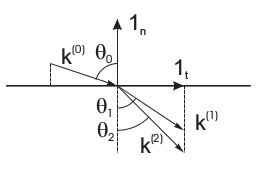
\includegraphics[scale=0.5]{ch5/image2}
	\captionof{figure}{ }
	\end{wrapfigure}
La dernière équation ressemble à la loi de Snell mais c'est plus compliqué car $k_1$ et $k_2$ sont
non-constants et dépendent de la direction de $\vec{k}^{(1)}$ et $\vec{k}^{(2)}$. On peut par contre
trouver les cosinus directeur à partir de l'équation de Fresnel si l'on connaît les cosinus directeur
de l'onde. Pour se faire, considérons le vecteur unitaire normal
\begin{equation}
\vec{1_n} = n_x\vec 1_x+n_y\vec 1_y+n_z\vec 1_z
\end{equation}
Et le vecteur unitaire dans le plan d'incidence tangentiel à la surface
\begin{equation}
\vec 1_t = t_x\vec{1_x}+t_y\vec{1_y}+t_z\vec{1_z}
\end{equation}
Selon la figure ci-essus, on peut écrire le vecteur d'onde de la première onde réfractée
\begin{equation}
\vec{k}^{(1)} = k^{(0)}\sin\theta_0\vec{1}_t+\sqrt{k^{(1)2}-k^{(0)2}\sin^2\theta_0}\vec{1_n}
\end{equation}
On en déduit les consinus directeurs
\begin{equation}
s_x = \frac{n^{(0)}}{n^{(1)}}t_x\sin\theta_0+n_x\sqrt{1-\frac{n^{(0)2}}{n^{(1)2}}\sin^2\theta_0},\qquad
s_y = \frac{n^{(0)}}{n^{(1)}}t_y\sin\theta_0+n_y\sqrt{1-\frac{n^{(0)2}}{n^{(1)2}}\sin^2\theta_0}
\end{equation}
\begin{equation}
s_z = \frac{n^{(0)}}{n^{(1)}}t_x\sin\theta_0+n_z\sqrt{1-\frac{n^{(0)2}}{n^{(1)2}}\sin^2\theta_0}
\end{equation}
En substituant cette équation dans l'équation de Fresnel, on trouve une équation transcendantale
(voir page 81, équation 5.19). Elle doit être résolue numériquement même si elle ne contient qu'une 
seule inconnue, $n^{(1)}$. Elle aura deux solutions acceptables : les indices de réfractions des
ondes réfractées. La direction peut être obtenue à l'aide des cosinus directeur calculée ci-dessus.



\section{Optical activity}
\subsection{Experimental Facts}
	\begin{wrapfigure}[7]{r}{4cm}
	\vspace{-8mm}
	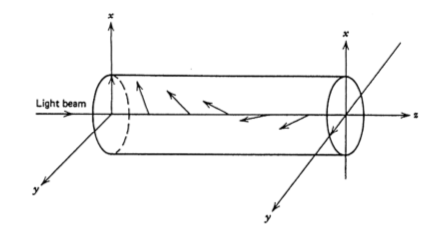
\includegraphics[scale=0.3]{ch5/image3}
	\captionof{figure}{ }
	\end{wrapfigure}
Dans certains milieux, on observe la rotation d'une polarisation linéaire en entrée au cours de 
la propagation. Il s'agit de l'\textbf{activité optique}, représentée ci-contre. Expérimentalement,
ce pouvoir de rotation est proportionnel à la longueur du milieu : on définit alors la \textit{puissance
de rotation} $\rho$ d'un milieu comme la rotation par unité de longueur. Si le sens de rotation est
horloger (en "regardant" la lumière venir) on parle de \textit{dextro-rotation} (sinon, \textit{
lévo-rotation}).

\newpage
\subsection{Macroscopic Theory of Optical Activity}
Nous avons étudié (chapitre 4) des matériaux caractérisés par l'équation constitutive
\begin{equation}
P =\epsilon_0\bar{\bar{\chi}}.E
\label{eq:5.20}
\end{equation}
ou il existe, pour chaque direction de propagation, deux modes propres qui peuvent se
propager. Ils sont polarisés linéairement et leur polarisation reste fixe en pendant qu'ils 
traversent le matériau.  Considérons une superposition de modes propres
\begin{equation}
D = \alpha D_0^{(1)}e^{i(\omega t-n^{(1)}k_0z)}+\beta D_0^{(2)}e^{i(\omega t-n^{(2)}k_0z)}
\end{equation}
Le retard de phase entre deux modes est donné par (voir \textit{Toolbox 2})
\begin{equation}
\Gamma = (n^ {(1)}-n^ {(2)})k_0z
\end{equation}
Il s'agit d'une fonction \textit{smooth}, continue en $z$. Ce type de variation ne correspond
pas à l'activité optique où la lumière est polarisée linéairement en chaque position ($\Gamma=
0$ ou $\pi$). En plus, \eqref{eq:5.20} n'autorise pas l'existence de l'activité optique. \\

L'activité optique est liée à la chiralité de la substance, et donc la différence entre la 
structure originale de la molécule et son image miroir. Les modes propres de tels matériaux ne
sont pas linéaires mais polarisés linéairement. Ceci est compatible avec la chiralité du 
matériel et l'absence d'un miroir plan. Considérons donc la superposition d'un mode de polarisation
circulaire gauche et droit
\begin{equation}
D(z=0) = \dfrac{D_0}{\sqrt{2}}\left[\dfrac{\sqrt{2}}{2}(\vec{1_x}+i\vec 1_y)e^{i\omega t} + 
\dfrac{\sqrt{2}}{2}(\vec 1_x-i \vec 1_y)e^{i\omega t}\right] = D_0e^{i\omega t}\vec{1_x}
\end{equation}
Ces deux modes ont pour indices $n_r$ et $n_l$, et donc des vitesses de propagation différentes (voir \textit{Toolbox 2}). 
Après propagation sur une distance $L$, on trouve
\begin{equation}
D(z=0) = \dfrac{D_0}{\sqrt{2}}\left[\dfrac{\sqrt{2}}{2}(\vec{1_x}+i\vec 1_y)e^{i\left(\omega t
-\frac{\omega}{c}n_rL\right)} + 
\dfrac{\sqrt{2}}{2}(\vec 1_x-i \vec 1_y)e^{i\omega t}\right]
\end{equation}
En regroupant les termes de même vecteur unitaire
\begin{equation}
D(z=L) = \dfrac{D_0}{2}e^{i\omega t}\left[\left(e^{-i\frac{\omega}{c}n_rL}+e^{-i\frac{\omega}{c}n_lL}
\right)\vec{1}_x+i\left(e^{-i\frac{\omega}{c}n_rL}-e^{-i\frac{\omega}{c}n_lL}\vec{1_y}\right)\right]
\end{equation}
En posant
\begin{equation}
\Phi = \frac{\omega}{c} \frac{n_l+n_r}{2},\qquad\qquad \rho = \frac{\omega}{c}\frac{n_r-n_l}{2}
\end{equation}
On peut réécrire $D(z=L)$ :
\begin{equation}
D(z=L) = D_0e^{i(\omega t-\Phi L)}\left(\cos\rho L\ \vec{1_x}+\sin\rho L\ \vec{1_y}\right)
\end{equation}
Il s'agit d'une onde polarisée \textbf{linéairement} pour toute les longueurs $L$, où $\rho$ est la 
\textbf{puissance de rotation}, reliée aux indices de réfraction des modes propres $(\rho>0$ : dextro, 
$\rho<0$ : levo). \\

Il faut maintenant essayer de généraliser les relations constitutives pour qu'un mode propre polarisé
circulairement soit possible. Pour se faire, on lui rajoute un terme en plus (c'est nouveau, on n'avait
pas ça avant)
\begin{equation}
p = \bar{\bar{\alpha}}.\epsilon_0E + \beta\dfrac{\partial H}{\partial t}
\end{equation}
où $\alpha$ est la polarisibilité.  Lorsque l'on rencontre cette relation constitutive, on retrouvera 
bien que la superposition de deux polarisation circulaires "opposées" résulte en une polarisation linéaire 
en rotation. Le dernier terme va causer l'apparition d'un $\beta \neq 0$ du à la structure hélicoïdale 
de la molécule. Le raisonnement est le suivant
\begin{enumerate}
\item La molécule est placée dans $\vec H(t)$
\item La variation du flux magnétique à travers la molécule génère un courant induit circulant autour
de $\vec H$ (loi de Faraday)
\item Molécule chirale : le courant induit crée une séparation des charges dépendante du temps, dans 
la direction de la dérivée temporelle de $\vec{H}$.
\item Il en résulte un moment dipolaire électrique
\item C'est le nouveau terme de notre expression
\end{enumerate}\ \\

En négligeant les interactions entre les moments dipolaires, le champ de polarisation s'obtient facilement
à partir de la densité de moment dipolaire
\begin{equation}
P = Np = N\left( \bar{\bar{\alpha}}.\epsilon_0E + \beta\dfrac{\partial H}{\partial t} \right)
\end{equation}
Avec la troisième loi de Maxwell (permettant d'écrire les fluctuations de $\vec{H}$ comme $\vec k \times
\vec E$) et en supposant un comportement linéaire des propriétés magnétiques, on peut éliminer la dérivée
temporelle
\begin{equation}
\vec P = n\vec P = N\bar{\bar{\alpha}}.\epsilon\vec  E+\dfrac{N\beta}{\mu_0}i\vec k\times \vec{E}
\end{equation}
En appliquant la définition du champ de déplacement électrique, on trouve
\begin{equation}
\vec D \equiv \epsilon\vec E+\vec P = \epsilon_0\vec +N\vec p = \epsilon_0\left(\bar{\bar{1}}+N
\bar{\bar{\alpha}}\right)\vec E + \epsilon_0\dfrac{N\beta}{\mu_0\epsilon_0}i\vec k\times\vec E =
\bar{\bar{\epsilon}}.\vec E+i\epsilon_0\vec G\times\vec E
\end{equation}
où $\vec G$ est un vecteur parallèle à la direction de propagation : c'est le \textbf{vecteur de giration}
(pseudo-vecteur\footnote{Voir page 85 pour la ré-écriture du tenseur $\bar{\bar{\epsilon}}'$ en fonction
de $G$, basé sur les propriétés des pseudo-vecteurs. C'est alors $\vec{G}$ qui contient \textbf{tous les
effets d'activité optique.}}). Le champ de déplacement est donc constitué de quelque chose proportionnel à
$\vec E$ et de quelque chose lié à la rotation de $\vec E$. L'activité optique est ainsi expliquée.\\

\subsection{An Application: The Polarimeter}
Lire rapidement le texte page 85-86. On utilise un polariseur et un analyseur pour déterminer l'angle de 
rotation de la polarisation linéaire causé par le milieu à activité optique.\\


La fin du chapitre est informatif (sur le dichroisme)